\documentclass[aip,pop,amsmath,amssymb,preprint,superscriptaddress]{revtex4-1} %preprint version
\usepackage{graphicx}% Include figure files
\usepackage{dcolumn}% Align table columns on decimal point
\usepackage{bm}% bold math

    \renewcommand{\topfraction}{0.9}    % max fraction of floats at top
    \renewcommand{\bottomfraction}{0.8}    % max fraction of floats at bottom
    \setcounter{topnumber}{2}
    \setcounter{bottomnumber}{2}
    \setcounter{totalnumber}{4}     % 2 may work better
    \setcounter{dbltopnumber}{2}    % for 2-column pages
    \renewcommand{\dbltopfraction}{0.9}    % fit big float above 2-col. text
    \renewcommand{\textfraction}{0.07}    % allow minimal text w. figs
    \renewcommand{\floatpagefraction}{0.7}    % require fuller float pages
    \renewcommand{\dblfloatpagefraction}{0.7}    % require fuller float pages
    \setlength{\abovecaptionskip}{5pt}
    \setlength{\belowcaptionskip}{5pt}
    \setlength{\parskip}{0pt}
    \setlength{\textfloatsep}{5pt} 

\begin{document}
\title{Potential signatures of dissipation from time-series analysis techniques using a turbulent laboratory MHD plasma}
\author{D.A. Schaffner}
\affiliation{Department of Physics, Bryn Mawr College, Bryn Mawr, PA 19010}
\author{M.R. Brown}
\author{A. Rock}
\affiliation{Department of Physics and Astronomy, Swarthmore College, Swarthmore, PA 19081}
\date{\today}
\begin{abstract}
The frequency spectrum of magnetic fluctuations as measured on the Swarthmore Spheromak Experiment (SSX) is broadband and exhibits a nearly Kolmogorov $5/3$ scaling. It features a steepening region which is indicative of dissipation of magnetic fluctuation energy similar to that observed in fluid and magnetohydrodynamic (MHD) turbulence systems. Two non-spectrum based time-series analysis techniques are implemented on this dataset in order to seek potential signatures of turbulent dissipation beyond the steepening of fluctuation spectra. Presented here are results for the flatness, permutation entropy, and statistical complexity, each of which exhibit a particular character at spectral steepening scales which can then be compared to the behavior of the frequency spectrum.
\end{abstract}
\maketitle

\section{Introduction}

Turbulent dissipation is an important topic in astrophysical and heliospheric plasmas. It involves long outstanding questions about the nature of the heliosphere including the solar corona heating problem and the radial temperature of the heliosphere. Despite decades of \textit{in-situ} observation of the solar wind, the exact process of how large scale kinetic and magnetic energy ejected from the sun gets transferred to the thermal motions of the plasma constituents remains unresolved~\cite{kiyani2015}. For highly collisional magnetic turbulence, resistivity of the plasma can fulfill the dissipation role as currents in the plasma deposit energy to particles through collisions (analogous to the role of viscosity in fluid turbulence)~\cite{biskamp2003,zhou2004}. However, in extremely sparse, hot and nearly collisionless plasmas such as the solar wind, resistivity cannot play such a role. The alternative mechanisms typically fall into two main groups: coupling between wave fluctuations and particle motion (including Landau damping or cyclotron resonance)~\cite{sahraoui2009} or though the formation of current sheets and reconnection layers which convert magnetic energy into kinetic flows, which can in turn be thermalized~\cite{osmin2014}.

In parallel with continued \textit{in-situ} exploration of these phenomena, production and analysis of magnetized turbulent plasma in the laboratory can be extremely useful for helping to understand what processes are possible in such a plasma and to what extent these various types of dissipation mechanisms are present or contribute to turbulent dissipation. While measurement of turbulent parameters in a laboratory plasma can have a variety of advantages over \textit{in-situ} satellite measurement (including higher spatial resolution and control of plasma parameter space), other diagnostic challenges do arise.  In this paper, we present a variety of analysis techniques aimed at identifying and characterizing potential turbulent dissipation signatures in a laboratory magnetically turbulent plasma—--the plasma wind tunnel in the Swarthmore Spheromak Experiment (SSX)~\cite{brown2014,brown2015a}. Previous results on SSX explore a system with a turbulent magnetic spectrum which exhibits a steepening indicative of the onset of some type of dissipation mechanism~\cite{schaffner2014a}. Follow-up work through detailed temporal and spatial spectral analysis along with arguments using anisotropy and reference to simulation strongly suggest that this steepening behavior is indeed reflective of some form of turbulent dissipation~\cite{schaffner2014c}. Examination of intermittent events and correlation with bursts of ion temperature suggest an intermittent mechanism may contribute to dissipation on SSX~\cite{schaffner2014b}. 

This manuscript presents a basic outline of two additional non-spectral based analysis techniques which can be studied at time scales consistent with the dissipation regime indicated by spectra, as well as discuss possible interpretations of the results in the context of dissipation mechanisms. More importantly however, this paper attempts to synthesize the results of multiple techniques in pursuit of a more holistic understanding of the nature of turbulent dissipation in this plasma.

Since turbulence is being explored in a laboratory setting, some clarification of the specific type of turbulence being investigated needs to be made. Laboratory-based plasma turbulence in the literature often refers to a system exhibiting broadband spectra of spatial and/or temporal fluctuations of plasma parameters including density, temperature and floating potential, within the framework of a stiff background magnetic field~\cite{brown2014}. It is associated with the formation and relaxation of gradients (such as pressure gradients in edge plasmas~\cite{zweben2007} or ion temperature gradients in fusion plasma cores~\cite{ghim2014}). In such systems, energy can be injected or dissipated at multiple scales, sometimes both occurring at the same scale~\cite{hatch2011}. In contrast, astrophysical plasmas exhibit turbulence that is more akin to fluid turbulence~\cite{goldstein1995}. That is, there tends to be a very large separation of energy injection scale and dissipation scale and typically no formation of large spatial gradients, nor a manifestation of non-local effects---particularly, the direct transfer of energy from a large scale to a small scale without passage through an intermediate scale such as has been observed in some laboratory work~\cite{moser2012}. Energy is injected at the largest scales of the system and energy is dissipated into heat at scales many orders of magnitude smaller. This genre of turbulence referred to as magnetohydrodynamic or MHD turbulence distinguishes it from the gradient-driven turbulence described above. Moreover, unlike conventional fluid turbulence, the collective behavior and interaction of plasma parameters makes MHD turbulence a significantly more challenging system to understand and characterize. Nevertheless, the largest MHD turbulence systems known exhibit Kolmogorov $5/3$ scaling of energy like that observed in conventional fluid turbulence~\cite{sahraoui2009,frisch1995}. 

The challenge in exploring this type of turbulence in the laboratory arises in how to faithfully reproduce the elements of MHD turbulence while avoiding formation of gradients. This requires avoiding typical laboratory plasma generation techniques including cathode sources and background fields. As will be described below, MHD turbulence is generated in SSX using plasma gun sources and flux-conserving boundaries which allow for the injection of turbulent magnetized plasma which can evolve dynamically without a background field. While plasma generated in this way cannot completely reproduce the conditions observed in heliospheric plasmas, it represents a closer approximation than other laboratory devices have been able to make.

\begin{figure}
\centerline{
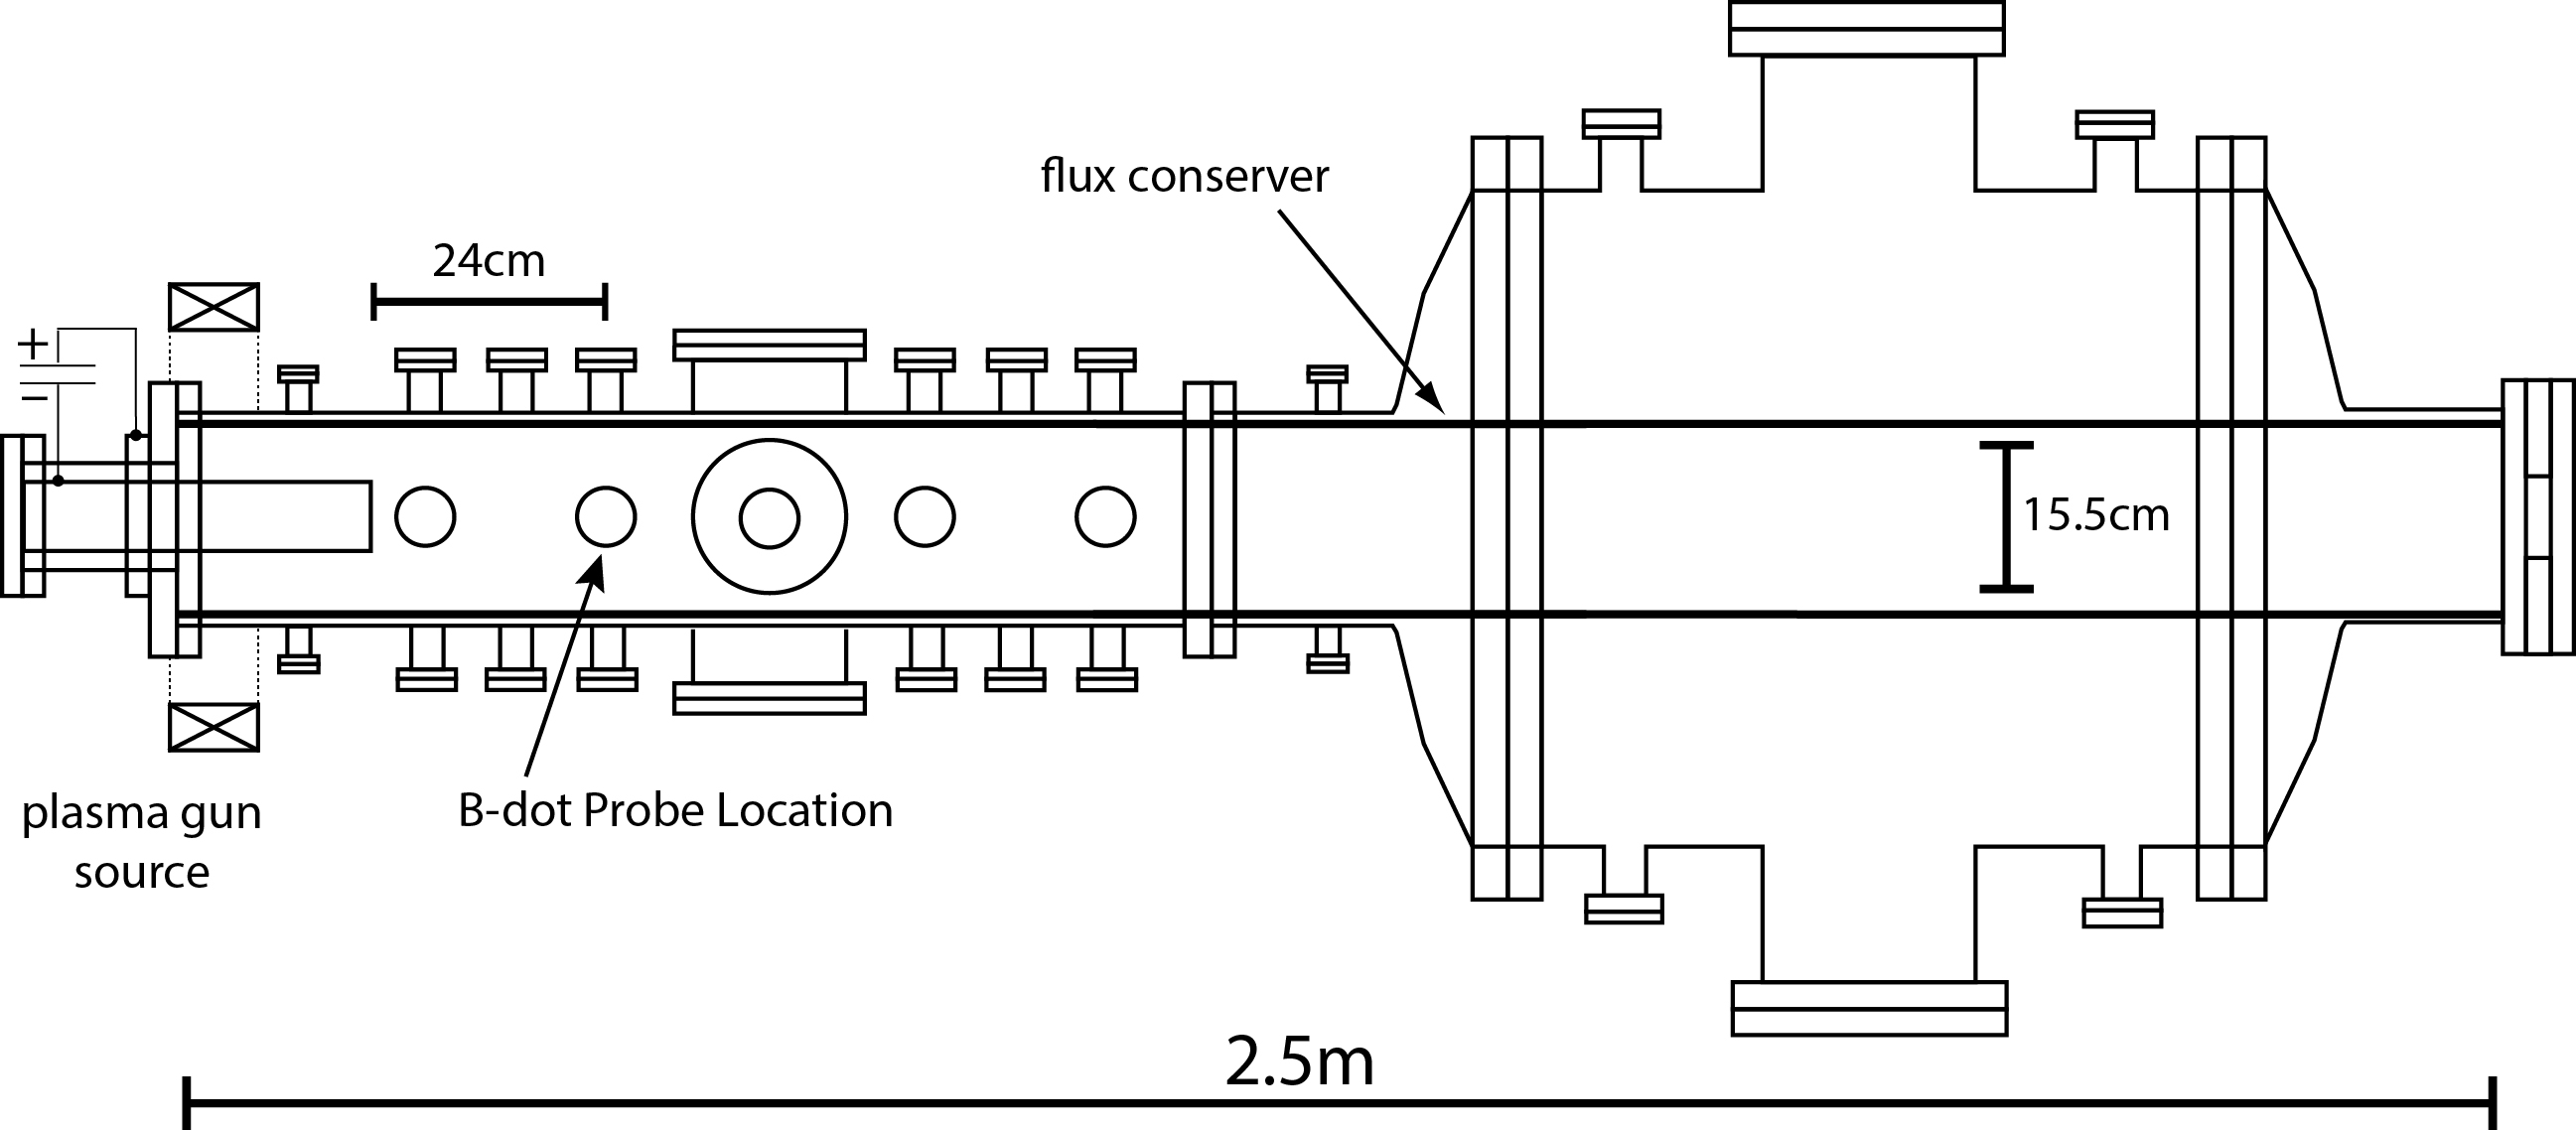
\includegraphics[width=8.5cm]{figure1.jpg}}
\caption{\label{fig:diagram} The expanded wind-tunnel configuration on the Swarthmore Spheromak Experiment, consisting of a 2.5m long by 15.5cm diameter, copper, flux-conserving cylinder. Plasma is launched using a plasma gun source at the far left and magnetic fluctuation measurements are made at a port 24cm from the end of the inner gun electrode. The triple axis probe has 3mm diameter loops and is inserted to a radial location 2.4cm off of the central axis.}
\end{figure}

\section{Combining Signatures of Turbulent Dissipation}

Since the model of scale-separated turbulence is best represented by an energy spectrum as a function of scale, the standard analysis tool is spectral decomposition of magnetic fluctuations. Ideally, fields could be measured spatially in order to decompose fluctuations into wavenumber space; however, most measurements are made at a single location, so temporal fluctuation spectra are used as a proxy, though turbulence theories generally do not make predictions for the behavior of such time spectra. If the turbulent system moves past the measurement point at a rate faster than the temporal change in the system, a direct correspondence can be made between temporal and spatial spectra---called the Taylor Hypothesis~\cite{deWit2013}. This procedure is done in the solar wind, for example, for measurements made in the at 1AU or beyond where solar wind velocities far exceed the temporal evolution scales. Such approximations cannot be as definitively made in this laboratory experiment where Alfven velocities ($\sim 140km/s$), which characterize the rate of temporal change of these plasmas, far exceed thermal or bulk flows ($\sim 20-40km/s$). Consequently, spectra are presented here as functions of measurement frequency rather than scale.

Nevertheless, the typical signature of turbulent dissipation extracted from either spatial or temporal spectra is a steepening of the spectrum at decreasing scale or increasing frequency just beyond the inertial range, which is itself characterized by Kolmogorov scaling (a scaling with the functional form of $k^{-5/3}$ or $f^{-5/3}$). This transition indicates an energy sink in the process. While within the inertial range, magnetic energy cascades from larger to smaller scales, but remains magnetic energy, beyond the inertial range, this magnetic energy is converted into other forms. In pure Kolmogorov theory, this energy becomes directly thermalized, but in more complicated plasma systems, the energy could conceivable be transferred into particle flows, coherent modes, or radiation, in addition to heat. These added complexities make interpretation of dissipation mechanisms with spectra alone potentially difficult. 

\begin{figure}
\centerline{
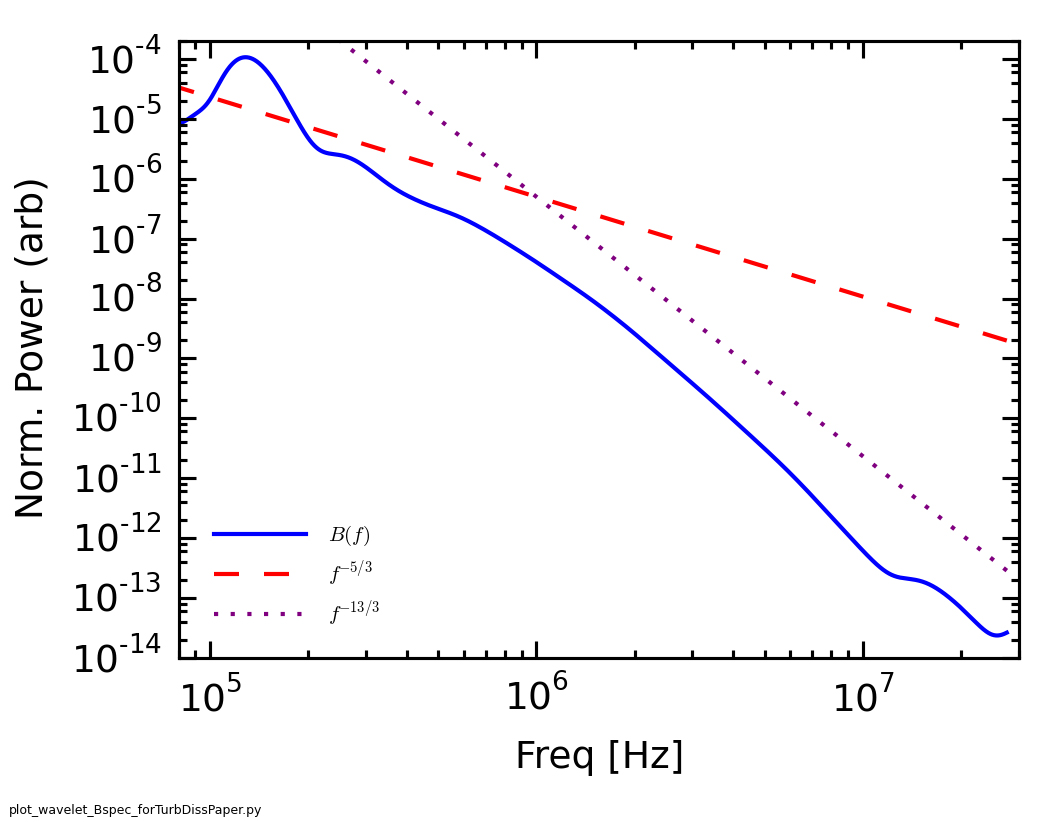
\includegraphics[width=8.5cm]{figure2.jpg}}
\caption{\label{fig:spectra} Fluctuation magnetic field spectrum on logarithmic axes consisting of the sum of $B_r$, $B_{\theta}$, and $B_z$, summed over fifty shots. The dashed orange line indicates Kolmogorov scaling ($f^{-5/3}$), while the dotted purple line indicates steeper scaling ($f^{-13/3})$.}
\end{figure}

\begin{figure}
\centerline{
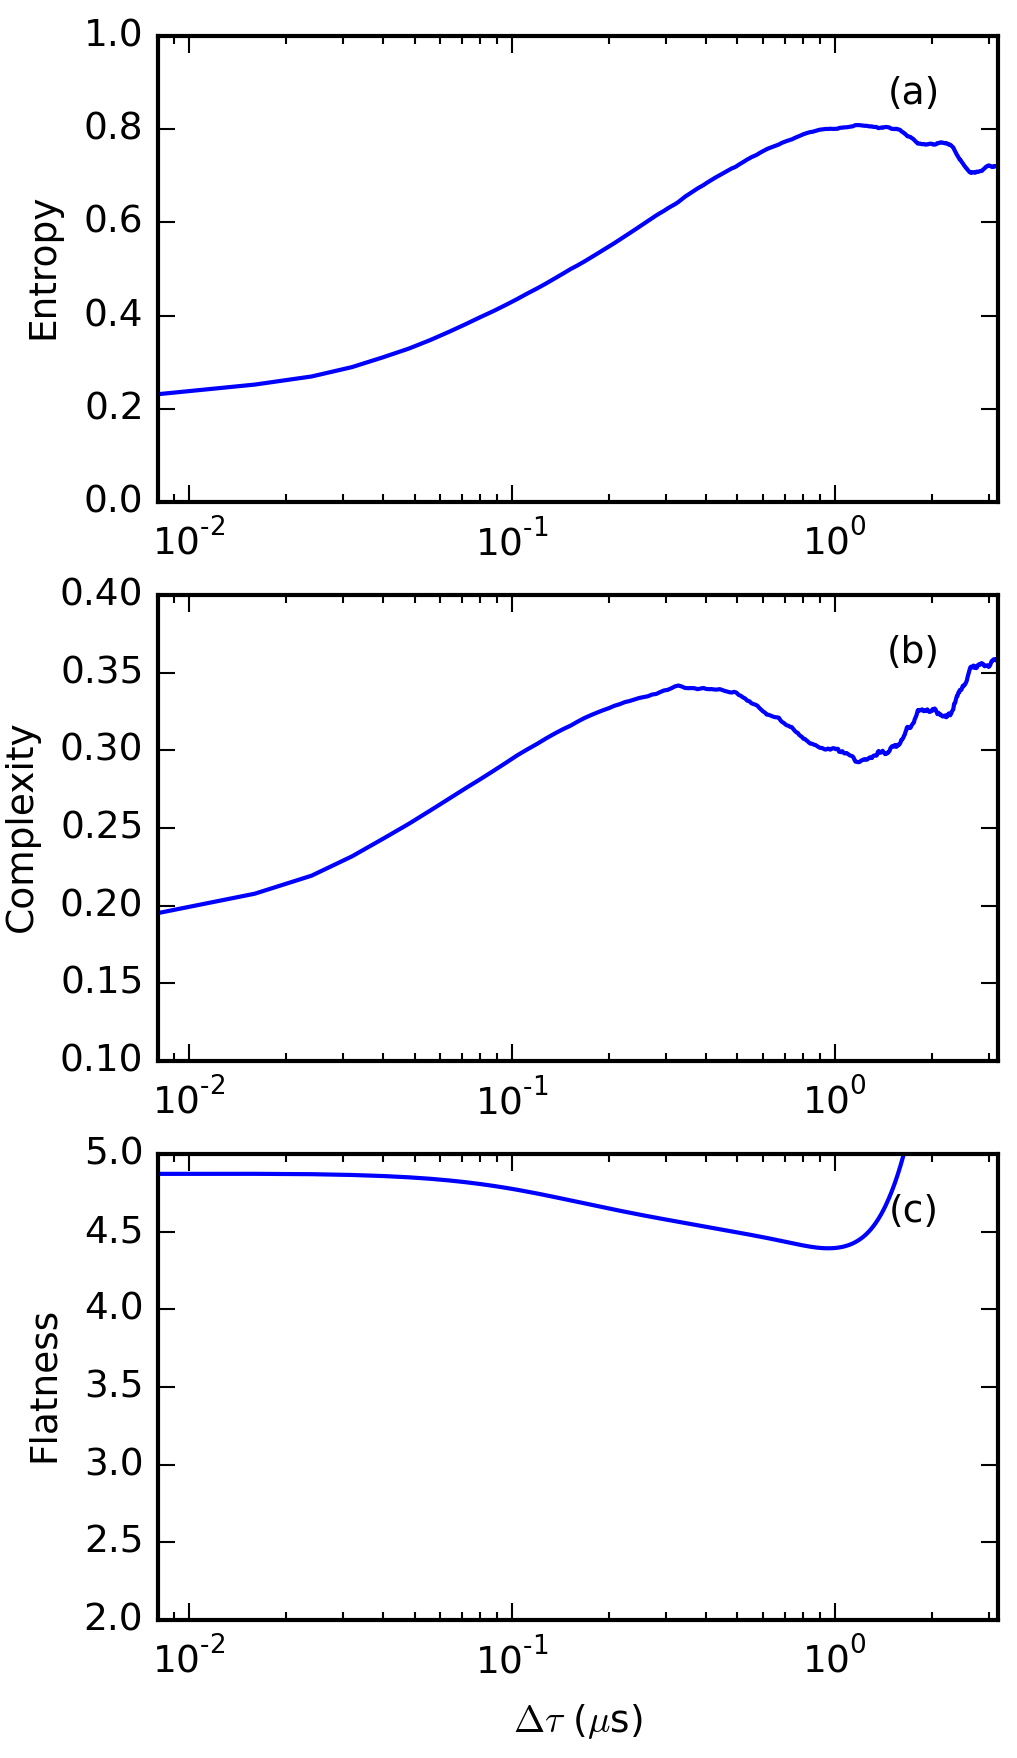
\includegraphics[width=8.5cm]{figure3.jpg}}
\caption{\label{fig:PESC}The permutation entropy (a), statistical complexity (b) and flatness (c), as a function of time scale, $\tau$.}
\end{figure}

Ultimately, the goal for the analyses presented here is to help determine the physical nature of the mechanism of the dissipation. While a steepening spectrum indicates the possibility of some type of dissipative mechanism occurring, it cannot immediately indicate the type of mechanism in question. The technique does provide some quantitative information. The location of the onset of steepening in wavenumber or frequency space can indicate the possible scale at which the mechanism operates (or begins to operate). In the solar wind, a steepening away from Kolmogorov scaling is seen to occur near scales associated with both the ion gyroradius, $\rho_{i}$, and the ion inertial length, $c/\omega_{pi}$~\cite{chen2014}. The scaling of the dissipation range can be informative, as well. For example, an observed scaling of $f^{-7/3}$ in the dissipation range could be indicative of the presence of a particular mode activity associated with the dissipation~\cite{shaikh2009}. It is here where comparison to the other analysis techniques can be illuminating. In particular, the intermittent character of the plasma can be explored using probability distribution functions (PDFs) of increments and structure functions. Observation of such intermittency can be indicative of the formation of current sheets or reconnection layers in the turbulent plasma which in turn hints at the mechanism converting magnetic energy into particle flows. Higher order structure function analysis can also be used to unearth the fractal scaling nature of the plasma~\cite{schaffner2015}. A relatively new technique called permutation entropy and statistical complexity~\cite{rosso2007} can also be used to explore a distinction between a chaotic versus a stochastic process. For instance, an increase in complexity might be associated with the non-linear interaction of linear modes~\cite{maggs2013,maggs2015}.

The remainder of this paper focuses on the application of the various analysis techniques described using the SSX plasma as a case study and examining their behavior at the time scales associated with turbulent dissipation in this plasma.

\section{Experimental Description}

The results presented in this paper are from measurements made in the extended MHD wind-tunnel configuration of the SSX. This mode of operation consists of a coaxial plasma gun source at one end of a $2.5$m long, $15.5$cm diameter copper cylinder, as indicated in Figure~\ref{fig:diagram}. The operation of the gun source has been described in previous work~\cite{brown2014}. For these results, the gun was operated with a stuffing flux of $1.3$mWb, and a discharge voltage of 4kV. Measurements of magnetic field fluctuations are measured using magnetic pick-up coils or B-dot probes. The data presented here is from a single location, $24$cm from the end of the gun source electrode, as indicated in the Figure, and 2.4cm away from the central axis of the cylinder. Plasma gun discharges persist on the order of $120\mu$s, but the analysis window for this data was restricted to $28$-$58\mu$s, where fluctuations are fairly stationary in the vicinity of the probe. Fifty shots are uses to generate an ensemble average for each analysis technique utilized. The shots are reproducible with a statistical spread on the order of $10\%$. Data is acquired using a Picoscope 5443A at 100MHz bandwidth, 1GB/s sampling and 14-bit channel depth.

\begin{table}
\begin{center}
\caption{\label{tab:params}Typical plasma parameters for this dataset.}
\begin{tabular}{cc}
$\langle |B|\rangle$&2500 G\\
$\Delta |B|/|B|$&0.2\\
$\langle n\rangle $&1.5$\times 10^{15} cm^{-3}$\\
$\langle T_{i}\rangle$&20 eV\\
$\langle T_{e}\rangle$&10 eV\\
$\beta$&0.3\\
$V_{alf}$&140 km/s\\
$V_{bulk}$&20-40km/s\\
$f_{ci}$&3.8 MHz\\
$\rho_{i}$&0.18 cm\\
$c/\omega_{pi}$&0.6 cm\\
$\lambda_{mfp}^{i}$&0.12 cm\\
\end{tabular}
\end{center}
\end{table}

\section{Analysis Techniques}

\subsection{Temporal Spectra}

The temporal spectrum is constructed by taking a Wavelet transform of the time range indicated using a sixth-order Morlet mother wavelet~\cite{brown2014}. Since the pickup probes actually measure $dB/dt$ directly, the spectra are converted into $B(t)$ by dividing each spectrum through by $f^2$. Each shot is transformed separately and then summed. The magnetic pickup probe measures three axes simultaneously---$B_{r}$, $B_{\theta}$, $B_{z}$ in the frame of the flux-conserving cylinder. Each axis spectrum is then summed to yield a total magnetic field spectrum.

\subsection{Flatness}
The normalized fourth-order structure function is defined as kurtosis or flatness~\cite{schaffner2015},
\begin{equation}
F(\tau) \equiv \frac{S^{4}(\tau)}{{(S^2(\tau))^{(2)}}}
\label{eq:structfunc}
\end{equation}
where $\tau$ is a time separation, $\Delta t$, at which the fourth-order structure function,
\begin{equation}
S^{4}(\tau) = \langle|B(t_{j}+\tau)-B(t_{j})|^{4}\rangle
\label{eq:structfunc2}
\end{equation}
is computed. Angle brackets indicate the average over $j$ time series elements. The time separation $\tau$ is increased linearly in increments of $0.08\mu s$. For reference, a Gaussian distribution will produce a flatness of F=3 for all values of $\tau$. Symmetric non-Gaussian distributions which exhibit super-Gaussian tails typically have flatness values of F$>$3. Each $\tau$ has a complementary frequency defined as $f = 1/\tau$. 

For this paper, the magnitude of the magnetic field as a function of time is constructed from each of the three axes by taking the square root of the sum of the squares. This magnetic magnitude then is scanned within the given time range for each value of $\tau$ in order to construct $F(\tau)$ for each shot. A total flatness curve is constructed by averaging over fifty shots. Since an increasing value of $\tau$ decreases the number of increments included in the structure function average, the analysis is limited to lower $\tau$'s and consequently higher frequencies. In this paper, the functional limit of the analysis is a $\tau = 1\mu s$. This constrains the range of interest to dissipation range fluctuations whose limits are defined by the spectrum analysis.

\subsection{Permutation Entropy and Statistical Complexity}

The PE/SC technique~\cite{bandt2002,rosso2007,weck2015} is initiated in a similar way to the construction of structure functions and flatness; the value of magnetic field is examined at a sequence of time points, but unlike a structure function where only two points are used, $n$ consecutive points are examined each separated by a time delay, $\tau$, defined in the same way as above. The value $n$ is often called the embedding dimension and $\tau$ the embedding delay. Rather than determining a difference in magnetic field at two points, an ordinal pattern constructed with field magnitudes at each of the $n$ time points is considered. Given $n$ time points, there can be $n!$ possible ordinal patterns or permutations. A given time series can be scanned to generate a distribution of ordinal patterns; since there is a maximal number of patterns, the probability of finding a given pattern in a dataset can be defined. This probability, $p$, then can be used to compute a Shannon entropy, or a permutation entropy~\cite{bandt2002},
\begin{equation}
S[P]  = -\sum^{n!} p(\pi) \log p(\pi)
\label{eq:pe}
\end{equation}
where $P$ is a distribution of $\pi$ encountered patterns. This quantity, $S[P]$, can be normalized to the maximal entropy and labeled as $H[P]$. Thus, the permutation entropy reflects the level of randomness in the distribution of ordinal patterns in a dataset. In other words, a dataset which exhibits equal amounts of all possible ordinal patterns is maximally permutation entropic and yields an $H[P] = 1$. A dataset with only one possible pattern (say a monotonically increasing ramp) would yield an $H[P] = 0$.

The utility of this metric can be expanded by examining not only the total probability of patterns, but also the distribution of patterns. That is, this metric asks the question: are certain patterns favored or forbidden? This tendency can be reflected by computing the disequilibrium of the distribution, a quantity which reflects how far from the uniform distribution a particular distribution is. Finally, the product of PE and disequilibrium can be constructed to form a quantity called the Jensen-Shannon complexity or statistical complexity~\cite{weck2015}, 
\begin{equation}
C = -2\frac{S \left[ \frac{P+P_e}{2} \right] - \frac{1}{2}S[P]-\frac{1}{2}S[P_e] }{\frac{N+1}{N} \log(N+1)-2 \log(2N)+\log(N)}H[P]
\label{eq:sc}
\end{equation}
where $P_e$ is the uniform distribution, $N=n!$, $H[P]$ is the normalized permutation entropy, and $S[P]$ the unnormalized permutation entropy. $C$ is normalized by construction~\cite{lamberti2004}.
Thus $C$ indicates a relative level of chaotic behavior in a time series; the lower the $C$, the more stochastic-like the time series, while the higher the $C$, the more chaotic-like the time series.

For this paper, the PE/SC analysis is computed using the magnetic field magnitude time series with an embedding dimension of $n=5$. An $H(\tau$) and $C(\tau$) is then constructed for the same series of $\tau$'s defined in the previous section. Similar to the flatness tool, the PE/SC analysis is limited to smaller values of $\tau$, so the functional limit of this metric is $1\mu s$ as well.

\section{Results}

Magnetic fluctuations between $28$ and $58\mu$s after discharge exhibit a broadband temporal spectrum between 100kHz and 10MHz as seen in Figure~\ref{fig:spectra}. Between about 200kHz and 1MHz, the spectra exhibits slightly steeper than Kolmogorov scaling which is indicated by the dashed orange line with a slope of $-5/3$. Beyond 1MHz, the spectrum steepens gradually indicating an increasing loss of magnetic fluctuation energy at higher fluctuations frequencies. The spectrum eventually reaches a slope of $-13/3$ indicated by the dotted purple line. Coherent modes appear at about 150kHz and 15MHz; the former mode is due to vibration of the gun field which appears later in the analysis period while the latter mode is due to the sloshing frequency of the LRC gun discharge circuit. Though the shift in the steepness of the curve is fairly gradual, for simplicity,  the frequency band between 200kHz and 1MHz is called the inertial range, and the band between 1MHz and 10MHz the dissipation range. The time scale range associated with 1MHz and 10MHz is 1$\mu$s to 0.1$\mu$s. This fluctuation spectrum is then compared to the analysis results for flatness, permutation entropy and statistical complexity. For the results of each of these, the direction of increasing frequency (to the right in Figure~\ref{fig:spectra}) corresponds to the direction of decreasing $\tau$ (to the left in Figure~\ref{fig:PESC}).

The flatness, $F(\tau)$, displayed in Figure~\ref{fig:PESC}(c), shows an increasing value with decreasing time scale between $\tau = 1\mu s$ and $\tau = 0.1\mu s$, which corresponds to the dissipation range of 1MHz to 10MHz. This indicates that the intermittency of the time series is steadily increasing the deeper it goes into the dissipation range (i.e. smaller $\tau$'s). The sharp spike in flatness at large time scales is likely due to the decreasing availability of statistics for the structure function computation.

The normalized permutation entropy, $H(\tau)$, on the other hand, shown in Figure~\ref{fig:PESC}(a), steadily decreases in the same range with decreasing $\tau$, going from a very large entropic value of 0.8 to a low entropic value of 0.2. This result appears to indicate that the randomness or stochasticity of the time series decreases steadily in the dissipation range.

Finally, the normalized statistical complexity, $C(\tau)$, shown in Figure~\ref{fig:PESC}(b), shows non-monotonic behavior in the region from $\tau = 1\mu s$ to $\tau = 0.1\mu s$. From the beginning of the inertial range, complexity begins to increase, suggesting an increase in chaotic behavior of the signal at dissipation range scales. The complexity peaks at a time scale of $\tau = 0.3\mu s$ which corresponds to a frequency of 3.33MHz. Beyond this scale, the complexity decreases for the remainder of the time range. The peaking of the complexity behavior in the dissipation range suggests that there is a scale in the system at which chaotic behavior is pronounced. It is intriguing that this peak resides near the average ion gyrofrequency for this plasma, at 3.8MHz. However, much more investigation needs to be made before asserting a connection between these two observations.

\section{Conclusions}

Magnetic fluctuation spectra in a laboratory turbulent MHD plasma is broadband and exhibits nearly Kolmogorov scaling up to a frequency of 1MHz. Beyond this point, an increasing slope is observed which is indicative of a dissipation mechanism in the system. The intermittency of the data is explored through the normalized fourth-order structure function called flatness and the relative stocasticity and complexity of the system is quantified using permutation entropy and statistical complexity. At the time scales corresponding to the dissipation region of the fluctuation spectrum, flatness increases monotonically, permutation entropy decreases monotonically, and statistical complexity decreases overall, but has a local maximum at a time scale of $0.3\mu s$ or corresponding frequency of 3.33MHz. 

These trends could be signatures of dissipation and when compared amongst one another, or to other analysis techniques, could illuminate particular mechanisms associated with the dissipation. For example, the observation of chaotic behavior at a particular scale could be correlated to the presence of a particular dissipation mechanism, including the intermittency implied by the non-Gaussian flatness values observed here, or perhaps to the generation of wave activity. Higher order structure function analysis reported previously for this laboratory plasma~\cite{schaffner2015} indicated a distinction in the fractal scaling behavior between dissipation and inertial range spectral regions; inertial range fluctuations exhibited multifractal behavior while dissipation range fluctuations exhibited monofractal behavior. The observation of increased complexity using the PE/SC technique corroborates this finding and supports that the dissipation mechanism in plasma has a chaotic nature, again, perhaps, in line with the generation and non-linear interaction of modes as suggested by work using this technique in edge turbulence~\cite{maggs2013}.

This work also highlights the limitation of these analyses with regard to time scale range. Ideally, longer time ranges with stationary turbulence would make for a better environment in which to explore these techniques. Unfortunately, the current setup on SSX is restricted in how close this ideal can be approached. However, efforts are underway to improve the experimental setup including the construction of a new plasma source at Bryn Mawr College which will focus on sustained plasma pulses to produce longer stationary datasets. Future work seeks to push the range of these techniques into the inertial range in order to explore the physics of the transition.

Finally, as reflected by the complicated and collective behavior of turbulent plasmas, the full understanding of turbulent dissipation may not be achievable with a single approach. Given this, many techniques should be explored and assimilated to produce a better picture of the nature of turbulent dissipation in plasmas.

\acknowledgements

This work was supported by grants from the Department
of Energy (OFES), and the National Science Foundation
(Physics Frontier Center for Magnetic Self Organization,
CMSO). The authors gratefully acknowledge the assistance of technicians
S. Palmer and P. Jacobs, and experimentalist Swarthmore undergraduate students Peter Weck'15 and Holden Parks'16.

\providecommand{\noopsort}[1]{}\providecommand{\singleletter}[1]{#1}%
\begin{thebibliography}{10}

\bibitem{kiyani2015} K.H. Kiyani, K.T. Osman, S.C. Chapman. {\it Phil. Trans. R. Soc. A} {\bf 373} 20140155 (2015).
\bibitem{biskamp2003} Biskamp, D. {\it Magnetohydrodynamic Turbulence.} Cambridge University Press, Cambridge, (2003).
\bibitem{zhou2004} Y. Zhou, W.H. Matthaeus, and P. Dmitruk. {\it Rev. Mod. Phys.} {\bf 76} 1015 (2004).
\bibitem{sahraoui2009} F. Sahraoui, M.L. Goldstein, P. Robert and Yu. V. Khotyaintsev. Evidence of a Cascade and Dissipation of Solar-Wind Turbulence at the Electron Gyroscale. Phys. Rev. Lett. {\bf 102} 231102 (2009).
\bibitem{frisch1995} Frisch, U. 1995, {\it Turbulence} (Cambridge: Cambridge Univ. Press).
\bibitem{osmin2014} K.T. Osman, W.H. Matthaeus, J.T. Gosling, A. Greco, S. Servidio, B. Hnat, S.C. Chapman, and T.D. Phan. {\it Phys. Rev. Lett.} {\bf 112} 215002 (2014).
\bibitem{schaffner2014a} D.A. Schaffner, V.S. Lukin, A. Wan, and M.R. Brown. Turbulence analysis of an experimental flux rope plasma. {\bf 56} 064003 (2014).
\bibitem{schaffner2014c} D.A. Schaffner, M.R. Brown and V.S. Lukin. ``Temporal and Spatial Turbulent Spectra of MHD Plasma and an Observation of Variance Anisotropy''. {\it ApJ} {\bf 790}, 126 (2014).
\bibitem{schaffner2014b} D.A. Schaffner, A. Wan, M.R. Brown. Phys. Rev. Lett. {\bf 112} 165001 (2014).
\bibitem{brown2014} M.R. Brown and D.A. Schaffner. ``Laboratory sources of turbulent plasma: a unique MHD plasma wind tunnel''. {\it Plasma Sources and Science Technology}. {\bf 23} 063001 (2014).
\bibitem{brown2015a} M.R. Brown and D.A. Schaffner. ``SSX MHD plasma wind tunnel''. {\it Journal of Plasma Physics}. (2015).
\bibitem{zweben2007} S. Zweben, J.A. Boedo, O. Grulke, C. Hildago, B. LaBombard, R.J. Maqueda, P. Scharin, and J.L. Terry. Plasma Phys. Control Fusion {\bf 49}, S1 (2007).
\bibitem{ghim2014} Y.-c. Ghim, A.R. Field, A.A. Schekochihin, E.G. Highcock, C. Michael, MAST team. Nucl. Fusion {\bf 54} 042003 (2014).
\bibitem{hatch2011} D.R. Hatch, P.W. Terry, F. Jenko, F. Merz, M.J. Pueschel, W.M. Nevins, and E. Wang. Phys. Plasmas {\bf 18}, 055706 (2011).
\bibitem{goldstein1995} M.L. Goldstein, D.A. Roberts and W.H. Matthaeus. Annu. Rev. Astron. Astrophys. {\bf 33} 283 (1995).
\bibitem{moser2012} A.L. Moser and P.M. Bellan. Nature. {\bf 482} 379 (2012).
\bibitem{deWit2013} T. Dudok de Wit, O. Alexandrova, I. Furno, L. Sorriso-Valvo, G. Zimbardo, {\it Space Sci. Rev.} {\bf 0038-6308} 1-29 (2013).
\bibitem{chen2014} C.H.K. Chen, L. Leung, S. Boldyrev, B.A. Maruca, and S.D. Bale. {\it Geophys. Res. Lett.} {\bf 41} 8081–8088 (2014).
\bibitem{shaikh2009} D. Shaikh and P.K. Shukla, 3D Simulations of Fluctuation Spectra in the Hall-MHD Plasma, Phys. Rev. Lett. {\bf 102}, 045004 (2009).
\bibitem{schaffner2015} D.A. Schaffner and M.R. Brown. {\it ApJ} 811:61 (2015).
\bibitem{bandt2002} C. Bandt and B. Pompe. Phys. Rev. Lett. {\bf 88} 174102 (2002).
\bibitem{rosso2007} O. A. Rosso, H.A. Larrondo, M.T. Martin, A. Plastino, and M.A. Fuentes, Phys. Rev. Lett. {\bf 99} 154102 (2007).
\bibitem{weck2015} P.J. Weck, D.A. Schaffner, and M.R. Brown. Phys. Rev. E {\bf 91} 023101 (2015).
\bibitem{lamberti2004} P.W. Lamberti, M.T. Martin, A. Plastino, and O.A. Rosso. Physica A. {\bf 334} 119 (2004).
\bibitem{maggs2013} J.E. Maggs and G.J. Morales. Plasma Phys. Control. Fusion {\bf 55} 085015 (2013).
\bibitem{maggs2015} J.E. Maggs, T.L. Rhodes, and G.J. Morales. Plasma Phys. Control. Fusion {\bf 57}  045004 (2015).

\end{thebibliography}
\end{document}
